\chapter{Revisão Bibliográfica} \label{cap2}

\corrigir{ Nesta seção serão} apresentadas duas subseções importantes para o entendimento deste trabalho, a revisão bibliográfica que trata de conceitos fundamentais ao entendimento do trabalho, e trabalhos relacionados que trata de outros trabalhos que são pertinentes à este.
	
\section{Fundamentação Teórica}
Nesta subseção tratamos de conceitos essenciais para o entendimento deste trabalho. Falaremos sobre alguns modelos matemáticos, critérios de estabilidade de sistemas discretos, projeto de controle por realimentação de estados, e métodos de identificação de sistemas e estimação de parâmetros, em especial identificação por mínimos quadrados e por subespaços.


\subsection{Modelos de Sistemas Dinâmicos}\label{capA}
O modelo matemático de um sistema dinâmico é uma forma de descrever uma parte do fenômeno físico que queremos controlar. Nesta seção serão apresentados alguns dos vários modelos matemáticos relacionados ao projeto.
\subsubsection{Equação Diferencial Ordinária}
Um sistema dinâmico pode ser modelado usando somente a descrição matemática do fenômeno desejado. Usamos como exemplo a modelagem do amortecimento em uma roda de um carro, visto na figura \ref{fig:modeloamortecimento}.

\begin{figure}
	\centering
	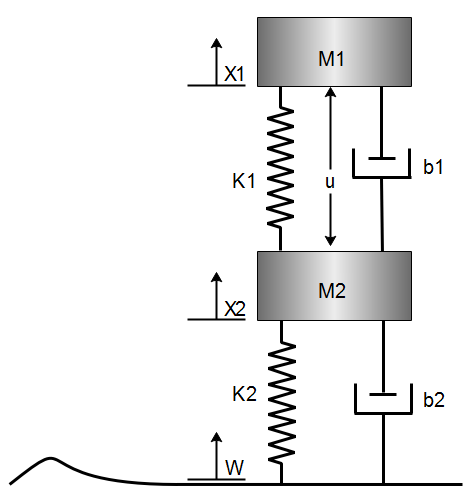
\includegraphics[width=0.5\linewidth]{modelo_amortecimento}
	\caption{Esquema do amortecedor da roda de um carro}
	\label{fig:modeloamortecimento}
\end{figure}

Onde $X_1$ e $X_2$ são a altura das massas $M_1$ e $M_2$, massa do carro e massa da roda, respectivamente. $K_1$ é o efeito elástico do amortecedor e $K_2$ é o efeito elástico da roda. $b_1$ é o efeito amortecedor da suspensão e $b_2$ é o efeito amortecedor da roda.
Esse sistema pode ser modelo em uma E.D.O. (Equação Diferencial Ordinária) usando as leis de Newton, visto nas equações \eqref{eq:edo1} e \eqref{eq:edo2}.

\begin{equation} \label{eq:edo1}
M_1 \ddot{X}_1=-b_1(\dot{X}_1-\dot{X}_2) -K_1(X_1-X_2)+U
\end{equation}
\begin{equation} \label{eq:edo2}
M_2 \ddot{X}_2=b_1 (\dot{X}_1 -\dot{X}_2) +K_1(X_1-X_2) +b_2(\dot{W} -\dot{X}_2)+K_1(W-X_2) -U
\end{equation}

\subsubsection{Funções de Transferência}
A função de transferência é uma equação que descreve o comportamento dinâmico de um sistema relacionando uma entrada com uma saída. Ela é a transformada de Laplace da resposta ao impulso do sistema.

Usando o mesmo sistema da figura \ref{fig:modeloamortecimento} e aproveitando as equações \eqref{eq:edo1} e \eqref{eq:edo2} podemos encontrar as equações de transferência referentes às saídas $X_1$ e $X_2$.

Aplicamos a transformada de Laplace nas equações $X_1$ e $X_2$ para obter:
\begin{equation} \label{eq:e2121}
(M_1s^2+b_1s+K_1) X_1(s) -(b_1s+K_1) X_2(s)=U(s)
\end{equation}
\begin{equation} \label{eq:e2122}
-(b_1s+ K_1) X_1(s) +(M_2s^2 + (b_1 + b_2)s +(K_1 + K_2))X_2(s)=(b_2s +K_2) W(s)-U(s)
\end{equation}
Fazendo as devidas manipulações matemáticas chegamos à função de transferência.
\begin{equation}\label{eq:e2123}
\begin{array}{c}
G_1(s)=\dfrac{X_1(s)-X_2(s)}{W(s)}= \dfrac{(M_1+M_2)s^2+b_2s+K_2} {\Delta}
\\
G_2(s)=\dfrac{X_1(s)-X_2(s)}{W(s)}= \dfrac{-M_1b_2s^3-M_1K_2s^2}{\Delta}
\\
\Delta=(M_1s^2+b_1s+K_1)\cdot (M_2s^2+ (b_1+b_2)s+(K_1+K_2))-(b_1s+K_1)\cdot (b_1s+K_1)
\end{array}
\end{equation}

Com as equações descritas em \eqref{eq:e2123} temos uma equação representando a transferência da entrada para a saída.
\subsubsection{Espaço de Estados}
A representação em espaço de estados é uma forma mais conveniente para representar sistemas no domínio do tempo quando existe mais de uma entrada ou saída do que a função de transferência. Um modelo linear é representado tipicamente no seguinte formato:
\begin{equation}\label{eq:ss}
\begin{array}{c}
\dot{x}=Ax+Bu\\
y=Cx+Du
\end{array}
\end{equation}
Onde $x \in \Re^n$ é o vetor de estado n-dimensional. $\dot{x}=dx/dt$, $u(t) \in \Re^p$ é o vetor de entradas formado por r funções temporais, $y(t) \in \Re^q$ é o vetor m-dimensional de saídas e $A \in \Re^{n\times n}$, $B \in \Re^{n \times p}$, $C \in \Re^{q \times n}$ e $D \in \Re ^{q \times p}$ são as matrizes do sistema constantes.


Podemos gerar uma representação de espaço de estados a partir da E.D.O. do sistema. Vamos utilizar novamente o sistema da figura \ref{fig:modeloamortecimento}. Definimos primeiramente os estados do vetor x, $x_1=X_1$, $x_2=\dot{X}_1$, $x_3=Y_1$ e $x_4=\dot{Y}_1$. Onde $Y_1=X_1-X_2$, geramos então as matrizes do espaço de estados usando as equações \eqref{eq:edo1} e \eqref{eq:edo2}:
\begin{equation}
A=\begin{bmatrix}
0 & 1 & 0 & 0\\
\dfrac{-b_1b_2}{M_1M_2} & 0 &\left[ \dfrac {b_1} {M_1} \left( \dfrac {b_1} {M_1} + \dfrac{b_1}{M_2} +\dfrac{b_2}{M_2} \right)- \dfrac{K_1}{M_1}\right] & \dfrac{-b_1}{M_1}\\
\dfrac{b_2}{M_2} & 0 & -\left( \dfrac{b_1}{M_1}+ \dfrac{b_1}{M_2}+ \dfrac{b_2}{M_2} \right) & 1\\
\dfrac{K_2}{M_2} & 0 & -\left( \dfrac{K_1}{M_1} +\dfrac{K_1}{M_2}+ \dfrac{K_2}{M_2} \right) & 0
\end{bmatrix}
\end{equation}
\begin{equation}
B=\begin{bmatrix}
0 & 0 \\
\dfrac{1}{M_1} & \dfrac{b_1b_2}{M_1M_2}\\
0 & \dfrac{-b_2}{M_2} \\
\left( \dfrac{1}{M_1}+ \dfrac{1}{M_2} \right) & \dfrac{-K_2}{M_2}
\end{bmatrix}
\end{equation}
\begin{equation}
\begin{bmatrix}
\dot{X}_1\\
\ddot{X}_1\\
\dot{Y}_1\\
\ddot{Y}_1
\end{bmatrix}
=
A
\begin{bmatrix}
X_1\\\dot{X}_1 \\Y_1 \\ \dot{Y}_1
\end{bmatrix}
+
B
\begin{bmatrix}
U\\W
\end{bmatrix}
\end{equation}
\begin{equation}
Y=
\begin{bmatrix}
0 & 0 & 1 & 0
\end{bmatrix}
\begin{bmatrix}
X_1\\\dot{X}_1\\Y_1\\\dot{Y}_1
\end{bmatrix}
+
\begin{bmatrix}
0 & 0
\end{bmatrix}
\begin{bmatrix}
U \\W
\end{bmatrix}
\end{equation}

\subsubsection{Modelo ARX}
O modelo ARX SISO linear tem o seguinte formato:
\begin{equation}\label{eq:ARXModel}
\begin{aligned}
y(t)+a_iy(t-1)+a_2y(t-2)+\dots+a_{na}y(t-na)=\\
b_1u(t)+b_2u(t-1)+\dots+b_{nb}u(t-nb+1)+e(t)
\end{aligned}	
\end{equation}

Onde y é a entrada, u é a saída e $e$ é o ruído. Isso implica que a saída $y(t)$ é uma predição a partir de uma média ponderada de entradas e saídas passadas. Os parâmetros $a_{na}$ e $b_{nb}$ podem ser estimados utilizando mínimos quadrados numa coleção de dados entrada-saída.

\subsection{Critérios de Estabilidade de sistemas discretos}

O conceito de estabilidade é extremamente importante para a análise de sistemas dinâmicos. Primeiramente definimos  estabilidade de acordo com mudanças nas condições iniciais. Consideremos a equação \eqref{eq:e22}.

\begin{equation} \label{eq:e22}
x(k+1)=f(x(k),k)
\end{equation}
Sejam $x_0(k)$ e $x(k)$ suas soluções quando as condições inicias são $x_0(k_0)$ e $x(k_0)$. Definimos:


$\bullet$ Estabilidade: A solução $x_0(k)$ é estável se para um dado $\epsilon>0$ existe um $\delta(\epsilon,k_0)$ tal que para todas as soluções com $||x(k_0)-x_0(k_0)||<\delta$ são tais que $||x(k)-x_0(k)||<\delta$ para todos os $k \geqslant k_0$.


$\bullet$ Estabilidade Assintótica: A solução $x_0(k)$ é assintoticamente estável se é estável e um $\delta$ pode ser escolhido tal que  $||x(k_0)-x_0(k_0)||<\delta$ que implica que $||x(k)-x_0(k)||\to\delta$ quando $k \to \infty$.


Existem outros tipos de estabilidade que são de interesse:


$\bullet$Estabilidade BIBO (Bounded-Input Bounded-Output): Um sistema linear invariante no tempo é definido BIBO estável se dado um sinal de entrada limitado ele produz uma saída limitada para cada valor inicial.


Dado que a estabilidade de um sistema é importante para o seu estudo, os métodos para determinar a sua estabilidade são de grande interesse. Os seguintes são alguns dos métodos utilizados para determinar a estabilidade de um sistema:
\begin{itemize}
	\item Cálculo dos autovalores da matriz A da representação de espaços de estado.
	\item Métodos baseados nas propriedades dos polinômios característicos.
	\item O método do lugar das raízes
	\item O método de Lyapunov
\end{itemize}

O cálculo dos autovalores de uma matriz de ordem maior que 2 à mão não é conveniente e em alguns casos é mais fácil calcular a equação característica da forma:
\begin{equation}
A(z)=a_0z^n+a_1z^{n-1}\dots+a_n=0
\end{equation}

E investigar suas raízes utilizando o método do lugar das raízes onde o critério de estabilidade muda para sistemas discretos determinando que para o sistema ser estável todas as raízes devem estar dentro do círculo unitário.

Outro método para determinar a estabilidade de um sistema é o critério de Jury, versão discreta do critério de Routh-Hourwitz. A tabela de Jury é formada da seguinte forma:
\begin{equation}
H(z)=\dfrac{b(z)}{a(z)}=\dfrac{b(z)}{a_0 z^n+a_1 z^{n-1}+\dots+a_n}
\end{equation}
\begin{equation}
\left|
\begin{matrix}
a_0 & a_1& \dots & a_n\\
a_n & a_{n-1}& \dots & a_0\\
b_0 & b_1 & \dots \\
b_{n-1} & b_{n-2} & \dots \\
c_0 & c_1 & \dots \\
\vdots & \vdots
\end{matrix}
\right.
\end{equation}
onde
\begin{equation}
\begin{matrix}
b_0=a_0- \dfrac{a_n}{a_0}a_n\\
b_1=a_1- \dfrac{a_n}{a_0}a_{n-1}\\
\vdots \\
b_k=a_k- \dfrac{a_n}{a_0}a_{n-k}\\
\vdots \\
c_k=b_k- \dfrac{b_{n-1}}{b_0}b_{n-1-k}\\
\end{matrix}
\end{equation}

Com a tabela formada aplicamos o critério de Jury que diz: se $a_0>0$, então todas as raízes estarão dentro do círculo unitário se e somente se todos os termos da primeira coluna das linhas impares forem positivos. Se nenhum elemento da primeira coluna das linhas impares for nulo, o número  de raízes fora do círculo unitário é igual ao número de elementos negativos.

O segundo método de Lyapunov é outra ferramenta útil para determinar a estabilidade de sistemas dinâmicos não lineares. A ideia é introduzir uma função de energia generalizada chamada função de Lyapunov que é zero no ponto de equilíbrio e positiva em outras posições. O equilíbrio será estável se pudermos mostrar que a função de Lyapunov diminui ao longo das trajetórias do sistema.


O primeiro passo é encontrar a função de Lyapunov definida como segue:


V(x) é uma função de Lyapunov do sistema
\begin{equation}\label{eq:lyap}
x(k+1)=f(x(k)) \qquad f(0)=0
\end{equation}

se:
\begin{enumerate}
	\item V(x) é contínuo em x e V(0)=0
	\item V(x) é definida positiva
	\item $\Delta V(x)=V(f(x))-V(x)$ é definida negativa
\end{enumerate}

Definimos:


$\bullet$Teorema de estabilidade de Lyapunov: A solução $x(k)=0$ é assintoticamente estável se existir uma função de Lyapunov para o sistema da equação \eqref{eq:lyap}. Se:
\begin{equation}
0<\varphi(||x||)<V(x)
\end{equation}
onde $\varphi(||x||)\to \infty$ quando $||x|| \to \infty$, então a solução é assintoticamente estável para todas as condições iniciais.


A grande dificuldade do teorema de Lyapunov é encontrar uma função de Lyapunov adequada. No entanto, para sistemas lineares como o da equação \eqref{eq:sis}, é fácil determinar uma função de Lyapunov quadrática.

\begin{equation} \label{eq:sis}
x_0(k+1)=\Phi x_0(k) \qquad x_0(0)=a_0
\end{equation}

Tomemos $V(x)=x^TP_x$ como candidato para a função de Lyapunov. O incremento de V é dado por:
\begin{equation}
\begin{array}{c}
\Delta V(x)=V(\Phi x)-V(x)=x^T\Phi ^T P \Phi x-x^TPx\\
=x^T(\Phi ^T P \Phi -P)x=-x^TQx
\end{array}
\end{equation}
Para que V seja uma função de Lyapunov é necessário e suficiente que exista uma matriz definida positiva P que satisfaça a equação \eqref{eq:lyapunov}.
\begin{equation}\label{eq:lyapunov}
\Phi ^T P \Phi - P= -Q
\end{equation}

\subsection{Projeto de Controlador com Realimentação de Estados}

Uma forma de controlar um sistema é utilizando realimentação de estados. A realimentação de estados é feita em sistemas modelado em espaço de estado e a cada instante cada estado individual é realimentado usando um ganho $K$. Esse tipo de controle requer que todos os estados sejam observáveis, entretanto, isso quer dizer que o sistema precisa de um sensor para cada estado conhecido o que acaba sendo muito custoso em termos de projeto e dinheiro. A solução para isso é projetar além do controlador um observador de estados, também chamado estimador, capaz de estimar o estado atual a partir da saída e da entrada do sistema.

\subsubsection{Controlador}

O controlador de realimentação de estados faz uma alocação de polos no sistema do tipo $A-BK$. Uma das formas de escolher K é com o seguinte procedimento explicado por Chen \cite{chen1998}:

\IncMargin{1em}
\begin{algorithm}[H]
	
	\Entrada{Matrizes A e B do sistema, polos escolhidos para serem alocados}
	\Saida{Ganho de realimentação de estados K}
	\Inicio{
	\nl	Crie uma matriz F com os autovalores (polos) escolhidos.\\
	\nl Selecione um vetor arbitrário $\hat{k}$ de forma que o par (F, $\hat{k}$) seja observável.\\
	\nl Solucione o $T$ único na equação de Lyapunov $AT-TF=B\hat{k}$.\\
	\nl Calcule o ganho de realimentação $K=\hat{k}T^{-1}$.
		
	}
	\Retorna{$K$}
	\label{alg:re}
	\caption{\textsc{Alocação de polos por realimentação de estados}}
\end{algorithm}
\DecMargin{1em}

\subsubsection{Estimador de Estados}

O estimador de estados é um processo que permite que medir os estados de um sistema a partir de sua entrada e saída. Um estimador deve ser projetado para que ele consiga obter os estados de um sistema o mais rápido possível dado a entrada e saída no momento anterior. Para isso fazemos a escolha dos polos do estimador de uma forma que eles reajam mais rápido que o sistema real, fazemos isso multiplicando a parte real dos polos escolhidos para o controlador por um número, efetivamente afastando eles do zero real. Uma forma de calcular o ganho $L$ do estimador de estados é muito similar ao algoritmo \ref{alg:re}:

\IncMargin{1em}
\begin{algorithm}[H]
	
	\Entrada{Matrizes $A$ e $C$ do sistema, polos escolhidos para serem alocados}
	\Saida{Ganho de realimentação de estados $L$}
	\Inicio{
		\nl	Crie uma matriz F com os autovalores (polos) escolhidos.\\
		\nl Selecione um vetor arbitrário $\hat{l}$ de forma que o par (F, $\hat{l}$) seja controlável.\\
		\nl Solucione o $T$ único na equação de Lyapunov $AT-TF=\hat{l}$C.\\
		\nl Calcule o ganho de realimentação $L=\hat{l}T^{-1}$.
		
	}
	\Retorna{$L$}
	\label{alg:ee}
	\caption{\textsc{Estimador de estados}}
\end{algorithm}
\DecMargin{1em}

Por fim, a equação \ref{eq:estimador} nos retorna os estados.

\begin{equation}\label{eq:estimador}
\begin{matrix}
\dot{z}=Az+Bu+(y-y_e)L
\end{matrix}
\end{equation}

\subsection{Identificação de Sistemas e Estimação de Parâmetros}
A maior parte das técnicas de controle aplicadas na indústria dependem do conhecimento de um modelo matemático do sistema a ser controlado. Apresentamos alguns dos modelos na seção \ref{capA} e nesta seção apresentaremos alguns dos métodos para obtermos os modelos matemáticos utilizados neste trabalho.


\subsubsection{Visão Geral}
A identificação de sistemas e estimação de parâmetros trata de métodos e práticas que permitem construir modelos dinâmicos de um sistema real a partir de experimentos . Muitas vezes um sistema construído que precisa ser controlado não pode ser modelado devido à limitações matemáticas ou imprecisão na interação dos componentes. Nestes casos utilizamos um método de identificação de sistemas para obter um modelo matemático. A identificação de sistemas se baseia em testar a resposta do sistema à certas entradas e a partir das respostas aproximar o modelo matemático de forma satisfatória.

\subsubsection{Escolha de sinais e estrutura}

A escolha dos sinais de entrada para a identificação de um sistema é importante pois a identificação deve ser capaz de medir o todo o alcance dinâmico do sistema. Se o sinal não for adequado identificamos um modelo que não é capaz de mostrar o funcionamento do sistema real. Uma condição para a escolha desses sinais é a condição PE (permanent excitement) \cite{katayama2005}, que dita que enquanto o sistema está submetido ao sinal ele está constantemente em dinâmica, sem chegar a estabilizar em um ponto. Um sinal que atende essa condição é o PRBS.


É importante escolher os sinais de interação com o sistema a ser identificado, levando em conta os atuadores presentes e os sensores disponíveis. Os sensores e o tipo de sistema estudado influenciam na escolha do tempo de amostragem de identificação, em sistemas lentos, como o controle de temperatura de uma sala, o tempo de amostragem pode ser longo, mas em sistemas rápidos como o controle da velocidade de um veículo o tempo de amostragem deve ser pequeno para possibilitar melhor controle. A escolha errada do tempo de amostragem pode fazer com que a identificação não funcione, pois limita a quantidade de dados obtidos do sistema e pode impedir a coleta de dados cruciais na mensuração da dinâmica do sistema.


A escolha da ordem do sistema também é de grande importância por causa do tipo de dinâmica que a ordem acarreta.

\subsubsection{Identificação por Mínimos Quadrados}
O método de mínimos quadrados é um dos mais conhecidos e utilizados em várias áreas da ciência e tecnologia. A partir de uma coleção de dados experimentais é possível encontrar um modelo matemático ARX.


Para um sistema SISO em que não conhecemos o seu modelo matemático podemos descrever o seu comportamento durante o teste como um conjunto de funções entrada-saída como na equação \eqref{eq:ARXModel}, pois à partir do conhecimento que temos da modelagem física do sistema podemos deduzir aproximadamente de quantos valores passados de y e de u o nosso sistema estudado depende.


Com os vetores entrada e saída em mão montamos uma matriz de regressores y e u no seguinte formato:
\begin{equation}
Y=\begin{bmatrix}
y(n) & y(n-1) & \dots & y(n-i) \\
y(n+1) & y(n) & \dots & y(n-i+1) \\
\vdots & \vdots & \ddots & \vdots\\
y(n+k) & y(n+k-1) & \dots & y(n+k-i) \\
\end{bmatrix}
\end{equation}

\begin{equation}
U=\begin{bmatrix}
 u(n) & u(n-1) & \dots & u(n-j)\\
 u(n+1) & u(n) & \dots & u(n-j+1)\\
 \vdots & \vdots & \ddots  & \vdots\\
 u(n+k) & u(n+k-1) & \dots & u(n+k-j)\\
\end{bmatrix}
\end{equation}

\begin{equation}\label{eq:regressores}
\psi=
\begin{bmatrix}
Y & U
\end{bmatrix}
\end{equation}

Onde $y(n-i)$ é o primeiro valor do vetor de saídas y e $u(n-i)$ é o primeiro valor do vetor de entradas u, i é a quantidade de regressores y que influenciam na saída y e j é a quantidade de regressores u que influenciam na saída y, $n+k$ é o número de valores do vetor de entrada.



Podemos então relacionar o vetor de saídas com a matriz de regressores A da seguinte forma:

\begin{equation}
\begin{array}{c}
\begin{bmatrix}
y_1 \\ y_2 \\ y_3\\ \vdots \\ y_n
\end{bmatrix}
=
\psi
\begin{bmatrix}
\theta_1 \\ \theta_2 \\ \vdots \\ \theta_n
\end{bmatrix}
\\
\hat{y}=\psi \hat{\theta}
\end{array}
\end{equation}
Onde $\hat{y}$ é um vetor que depende da matriz de regressores A e do vetor $\hat{\theta}$. Conhecemos $\hat{y}$ e A, queremos determinar $\hat{\theta}$. Desde que X seja não singular é possível determinar o vetor de parâmetros invertendo a matriz:
\begin{equation}\label{eq:MQ}
\theta=\psi^{-1}y
\end{equation}

A matriz $\psi$, no entanto, não é invertível e para realizarmos $\psi^{-1}$ utilizamos a pseudo inversa, que será utilizada em diversas partes desse trabalho, representada por $\{ \cdot\}^\dagger$, onde $\{\cdot\}$ é a matriz que receberá a operação pseudo inversa.
\begin{equation}
A^\dagger=[A^TA]^{-1}A^T
\end{equation}

E a equação \eqref{eq:MQ} se torna:
\begin{equation}\label{eq:MQ2}
\theta=\psi^\dagger y
\end{equation}


A equação \eqref{eq:MQ} é a única equação que satisfaz todos os regressores do sistema de equações formado a partir da equação \eqref{eq:ARXModel}. Assumindo que conhecemos $\hat{\theta}$ e que existe um resíduo $\xi$ entre o valor observado y e o valor obtido a partir do vetor de regressores $\psi$ da forma:
\begin{equation}\label{eq:eMQxi}
y=\psi^T\hat{\theta}+\xi
\end{equation} 

Este resíduo é o menor possível devido ao fato de que a equação \eqref{eq:MQ2} ser demonstravelmente minimizada.


Apresentamos aqui um pseudo algoritmo para a identificação por mínimos quadrados:

\IncMargin{1em}
\begin{algorithm}[H]

	\Entrada{Vetor de entradas $U[N]$, vetor de saídas $Y[N]$, quantidade de regressores de $Y$ $n$, quantidade de regressores de $U$ $m$}
	\Saida{Vetor $\hat{\theta}$}
	\Inicio{
		Faça a matriz de regressores $psi$ da equação \eqref{eq:regressores}\\
		Calcule $\theta$ com a equação \eqref{eq:MQ2}
	}
	\Retorna{$\theta$}
	\label{alg:mq}
	\caption{\textsc{Identificação por Mínimos Quadrados}}
\end{algorithm}
\DecMargin{1em}


%
%\subsubsection {Filtro de Kalman}
%O filtro de Kalman, também conhecido como estimador linear quadrático, é um algoritmo que utiliza uma série de medidas tomadas ao longo do tempo, que contém ruídos e outros tipos de erros, e produz um estimador capaz de estimar com maior confiança um certo valor. Ele é utilizado em uma grande variedade de aplicações de engenharia, como localização GPS e navegação, sua aplicação mais famosa foi no programa espacial Apollo, e é um tópico especialmente importante para a teoria de sistemas de controle, devido a sua capacidade de estimação de sistemas não lineares.
%\paragraph{Visão Geral}
%O filtro de Kalman utiliza um modelo dinâmico de um sistema, suas entradas de controle, e medidas de sensores para gerar uma estimativa das grandezas medidas do sistema. Usando um modelo recursivo para obter as estimativas, medidas passadas, ele consegue obter uma estimativa mais fiel ao sistema real do que utilizando somente uma medida. O filtro funciona em duas etapas, uma de propagação, onde se utiliza a estimativa do estado anterior para se obter uma estimativa do estado atual, e uma de assimilação, onde a estimativa do estado atual é combinada com a observação do estado real para se obter um modelo de estimativa mais preciso. 
%
%
%Usaremos a nomenclatura de Aguirre, onde $t_1$ é substituído pela iteração atual indicada por k, e o $t_2$ é substituído pela próxima iteração k+1. A notação ($t_1$|$t_1$) é substituída por um sinal '+' para indicar o instante $t_i$ após ter sido incluída a informação em $t_i$. Da mesma forma será utilizado um sinal '-' para indicar a grandeza que se refere ao instante $t_i$ antes de ter sido incluída a informação referente àquele instante. A equação que rege a propagação é a seguinte:
%\begin{equation} \label{eq:prop}
%\hat{x}^{-}_{k+1}=\Phi_k \hat{x}^+_k+\Gamma_ku_k
%\end{equation}
%
%\paragraph{Etapa de propagação}
%Conhecendo a função de densidade de probabilidade de $x_k^+$, indicada por $f_k\sim \mathcal{N}(\bar{x}^+_k, P^+_k)$, deseja-se encontrar a função de densidade de probabilidade de $x^-_{k+1}$. Ou seja, na etapa de propagação deseja-se saber o que acontece à $f_k$ ao ser propagado pela equação \eqref{eq:prop}. Assumimos que $f_k$ é gaussiana e portanto $f_-$ também será, deste modo basta determinar $\bar{x}^-_{k+1}$ e $P_-^{k+1}$ contidos em $f_- \sim \mathcal{N}(\bar{x}^-_{k+1},P^-_{k+1})$ para caracterizar $f_-$.
%
%
%Segundo Aguirre \cite{aguirre2015} encontramos:
%\begin{equation}
%\bar{x}^-_{k+1}=\Phi_k\bar{x}^+_k+\Gamma_ku_k
%\end{equation}
%\begin{equation}
%P^-_{k+1}=\Phi_kP^+_k\Phi^T_k+\Upsilon_kQ_k\Upsilon^T_k
%\end{equation}
%
%A equação mostra que ao longo da etapa de propagação a incerteza aumenta devido à presença de ruído no modelo dinâmico usado.
%
%\paragraph{Etapa de assimilação}
%Vimos que na etapa de propagação o vetor de estado $x^+_k$ é propagado para a próxima iteração resultando em $x^-_{k+1}$. A segunda etapa, a de assimilação, ocorre com a chegada de nova informação na iteração k+1. O objetivo é a determinação de $f_+ \sim \mathcal{N} (\bar{x}^+_{k+1},P^+_{k+1})$ a partir de $f_-$ e da medição na iteração $y_{k+1}$. De forma semelhante à etapa de propagação, devemos encontrar $\bar{x}^+_{k+1}$ e $P^+_{k+1}$. Após os devidos passos encontramos:
%\begin{equation}
%\bar{\mathbf{x}}^+_{k+1}=\bar{\mathbf{x}}^-_{k+1}+K_{k+1}[\mathbf{y}_{k+1}-H_{k+1} \bar{\mathbf{x}} ^-_{k+1}]
%\end{equation}
%\begin{equation}
%P^+_{k+1}=P^-_{k+1}-K_{k+1} H_{k+1} P^-_{k+1}
%\end{equation}
%\begin{equation}
%K_{k+1}=P^-_{k+1} H^T_{k+1}[H_{k+1} P^-_{k+1} H^T_{k+1}+R_{k+1}]^-1
%\end{equation}
%
%Com estas equações completamos o conjunto de equações necessárias para entender o filtro de Kalman.

\subsubsection {Identificação por Subespaços}
A identificação por subespaços é um algoritmo, que, a partir de uma sequência de dados experimentais, é capaz de gerar um modelo em espaço de estados. O procedimento aqui descrito é explicado com mais detalhes por Rico \cite{ricco2012}.


Com o sistema a ser identificado em mãos precisamos executar um ou mais experimentos medindo o sinal de entrada e o sinal da saída do sistema. Para que a identificação funcione adequadamente o sinal de entrada deve atendar a condição de persistência de excitação \cite{katayama2005}, um sinal binário pseudo aleatório atende esse requisito.


Aplicamos o sinal no sistema e medimos a sua resposta ao longo de um tempo $t$ com um tempo de amostragem $t_s$ e obtemos dois vetores, $u[N]$, sinal PRBS de entrada aplicados ao sistema, e $y[N]$ que é a saída medida do sistema, $N$ é a quantidade de medidas tomadas. Com esses dois vetores geramos um conjunto de 4 matrizes em blocos de Hankel.

\begin{equation}\label{eq:matrizhankel}
U_{0|2i-1}=
\begin{pmatrix}
u_0 & u_1 & \dots & u_{j-1} \\
u_1 & u_2 & \dots & u_{j} \\
\vdots & \vdots & \ddots & \vdots\\
u_{i-1} & u_i & \dots & u_{i+j-2}\\
\hline
u_i & u_{i+1} & \dots & u_{i+j-1}\\
u_{i+1} & u_{i+2} & \dots & u_{i+j}\\
\vdots & \vdots & \ddots & \vdots\\
u_{2i-1} & u_{2i} & \dots & u_{2i+j-2}
\end{pmatrix}
=\dfrac{U_p}{U_f}
\end{equation}

Onde $i=nm$, n é a ordem da matriz em blocos de Hankel desejada e m é o número de entradas, e $j=N-2i+1$, $U_f$ é a matriz em blocos das entradas futuras, $U_p$ é a matriz em blocos das entradas passados. O mesmo é feito para $y[N]$ gerando $Y_f$ e $Y_p$. Com essas matrizes em mãos geramos $W_p=[U_p~~Y_p]^T$ e podemos encontrar $O_i$ fazendo:
\begin{equation}\label{eq:oi}
O_i=Y_{f/U_f} W_p
\end{equation}

$Y_{f/U_f}W_p$ denota uma projeção oblíqua de $Y_f$ sobre $W_p$ ao longo de $U_f$ calculado por:

\begin{equation}\label{eq:oiexp}
O_i=[Y_f/U_f^\perp][W_p/U_f^\perp]^\dagger W_p
\end{equation}

Em seguida fazemos uma decomposição SVD de $O_i$:

\begin{equation}\label{eq:svd}
O_i=USV^T=\begin{pmatrix}
U_1 &U_2
\end{pmatrix}\begin{pmatrix}
S_1 & 0\\ 0 & 0
\end{pmatrix} 
\begin{pmatrix}
V_1^T \\ V_2^T
\end{pmatrix}
\end{equation}

Com $O_i$ decomposto calculamos $\Gamma_i$ da seguinte forma:
\begin{equation}\label{eq:gammai}
\Gamma_i=U_1 S_1^{1/2}
\end{equation}

Tiramos a raiz quadrada de uma matriz com o seguinte procedimento:
\begin{equation}
A=QPQ^{-1}
\end{equation}
Onde $Q$ e $P$ fazem uma decomposição de $S_1$ e $P$ é escolhido de forma que se conheça a sua raiz quadrada.
\begin{equation}
S_1=(QP^{1/2}Q^{-1})^2
\end{equation}
\begin{equation} \label{eq:raizs1}
S_1^{1/2}=QP^{1/2}Q^{-1}
\end{equation}

Com $\Gamma_i$ em mãos podemos identificar as matrizes $A$ e $C$ do sistema. $\Gamma_i$ é equivalente à matriz de observabilidade do sistema, então $C$ é a primeira linha de $\Gamma_i$ e $A$ pode ser encontrado por:
\begin{equation}\label{eq:matriza}
A=\underline{\Gamma_i^\dagger}\overline{\Gamma_i}
\end{equation}

Onde a matriz sublinhada significa que foi removida a última linha e a matriz sobrelinhada significa que foi removida a primeira linha.


Encontramos $B$ e $D$ com a equação:

\begin{equation}
\Gamma_i ^\perp Y_f U_f ^\dagger=\Gamma_i ^\perp H^d_i
\end{equation}

Renomeamos os termos dessa equação da seguinte forma:
\begin{equation}
Q=\begin{pmatrix}
D& 0 & 0 & \dots & 0\\
CB & D & 0 & \dots & 0\\
CAB & CB & D & \ddots & 0\\
\vdots & \vdots & \vdots & \ddots & \vdots\\
CA^{i-2}B & CA^{i-3}B & CA^{i-4}B& \dots & D
\end{pmatrix}
\end{equation}
\begin{equation}
\begin{pmatrix}
M_1 & M_2 & \dots & M_i
\end{pmatrix}
=
\begin{pmatrix}
L_1 & L_2 & \dots & L_i
\end{pmatrix}Q
\end{equation}

Reescrevemos essa equação:

\begin{equation} \label{eq:eqdb}
\begin{pmatrix}
M_1\\M_2\\ \vdots \\ M_i
\end{pmatrix}
=
\begin{pmatrix}
L_1 &L_2& \dots & L_{i-1}& L_i\\
L_2& L_3 & \dots & L_i & 0\\
L_3 & L_4 & \dots & 0 & 0\\
\vdots & \vdots & \ddots & \vdots & \vdots\\
L_i & 0 & \dots & 0 &0
\end{pmatrix}
\begin{pmatrix}
I_l & 0 \\ 0 & \underline{\Gamma_i}
\end{pmatrix}
\begin{pmatrix}
D \\ B
\end{pmatrix}
\end{equation}

E dessa forma obtemos todas as matrizes do sistema identificado.

\paragraph{Algoritmos}\label{s:subalgoritmos}
Para facilitar o entendimento colocamos em forma de algoritmo os passos que devem ser tomados para identificar um sistema por subespaços.

\IncMargin{1em}
\begin{algorithm}[H]
	\Entrada{Vetor de entradas $U[N]$, vetor de saídas Y[N], ordem determinada do sistema n}
	\Resultado{Matrizes do espaço de estados do sistema A, B, C e D}
	\nl Gerar as matrizes de bloco de Hankel $Y_p$, $Y_f$, $U_p$ e $U_f$, usando a equação \eqref{eq:matrizhankel}\\
	\nl Calcular $O_i$ usando as equações \eqref{eq:oi} e \eqref{eq:oiexp}\\
	\nl Decomposição SVD de $O_i$ \eqref{eq:svd}\\
	\nl Calcular $\Gamma_i$ \eqref{eq:gammai}\\
	\nl Obter A e C \eqref{eq:matriza}\\
	\nl Obter B e D \eqref{eq:eqdb}\\
	\Retorna{$A$, $B$, $C$, $D$}
	\label{alg:sub}
	\caption{\textsc{Identificação por Subespaços}}
	
\end{algorithm}
\DecMargin{1em}

\subsubsection{Validação de modelos identificados}

Não basta identificar o modelo usando os métodos descritos anteriormente para que ele seja adequado ao sistema real, é preciso validar o modelo obtido usando técnicas capazes de medir o desempenho do modelo.


A técnica que será utilizada é descrita por Aguirre \cite{aguirre2015}, chamada análise de resíduos, onde é feita uma auto correlação dos resíduos, diferença entre a saída real do sistema e a saída do modelo obtido para um mesmo sinal, para verificar a brancura desse sinal. Quanto menos auto correlacionado melhor, pois significa que o resíduo se assemelha a ruído branco.

\section{Trabalhos Relacionados}


A identificação de sistemas por caixa-preta, especificamente por subespaços é um tema recorrente do estudo da engenharia, dado que é uma forma de identificar um sistema complexo com menos trabalho mental na modelagem matemática dos fenômenos físicos.


Em 2009, Jernigan et al. \cite{jernigan2009}, publicaram um artigo falando sobre uma experiência que fizeram na construção e utilização de uma experiência de laboratório remota. Eles escolheram como experimento a levitação de uma bola de praia de plástico usando um soprador de ar. Um grupo de alunos foi encarregado de modelar, simular e controlar o sistema usando o laboratório remoto. \melhorar{ Este trabalho foi essencial para o nosso entendimento da modelagem da levitação de uma bola por fluxo de ar e especialmente do tipo de medida necessária para criar um simulador do sistema. Diferente deste trabalho Jernigan et al. não fez identificação do sistema e optou por fazer modelagem matemática.}


Em 2017, Chacon et al. \cite{chacon2017}, relatam em um artigo a construção de um túnel de vento para o ensino de engenharia de controle. Eles tem o mesmo objetivo deste trabalho em relação à construir uma plataforma de experimentos barata e reprodutível mas diferem porque aplicam a plataforma para aprendizado à distância. No artigo eles descrevem um processo de identificação caixa preta usando um sinal binário pseudo aleatório bastante parecido com o que será utilizado neste trabalho, mas tratam a identificação como um exercício a ser aplicado aos alunos.



% Fim Capítulo















